\Chapter{Megvalósítás}

% Ez a fejezet mutatja be a megvalósítás lépéseit.
% Itt lehet az esetlegesen előforduló technikai nehézségeket említeni.
% Be lehet már mutatni a program elkészült részeit.

% Meg lehet mutatni az elkészített programkód érdekesebb részeit.
% (Az érdekesebb részek bemutatására kellene szorítkozni.
% Többségében a szöveges leírásnak kellene benne lennie.
% Abból lehet kiindulni, hogy a forráskód a dolgozathoz elérhető, azt nem kell magába a dolgozatba bemásolni, elegendő csak behivatkozni.)

% A dolgozatban szereplő forráskódrészletekhez külön vannak programnyelvenként stílusok.
% Python esetében például így néz ki egy formázott kódrészlet.
% \begin{python}
% import sys

% if __name__ == '__main__':
%     pass
% \end{python}

% A stílusfájlok a \texttt{styles} jegyzékben találhatók.
% A stílusok között szerepel még C++, Java és Rust stílusfájl.
% Ezek használatához a \texttt{dolgozat.tex} fájl elején \texttt{usepackage} paranccsal hozzá kell adni a stílust, majd a stílusfájl nevével megegyező környezetet lehet használni.
% További példaként C++ forráskód esetében ez így szerepel.
% \begin{cpp}
% #include <iostream>

% class Sample : public Object
% {
%     // An empty class definition
% }
% \end{cpp}
% Stílusfájlokból elegendő csak annyit meghagyni, amennyire a dolgozatban szükség van.
% Más, C szintaktikájú nyelvekhez (mint például a JavaScript és C\#) a Java vagy C++ stílusfájlok átszerkesztésére van szükség.
% (Elegendő lehet csak a fájlnevet átírni, és a fájlban a környezet nevét.)

% Nyers adatok, parancssori kimenetek megjelenítéséhez a \texttt{verbatim} környezetet lehet használni.
% \begin{verbatim}
% $ some commands with arguments
% 1 2 3 4 5
% $ _
% \end{verbatim}

% A kutatás jellegű témáknál ez a fejezet gyakorlatilag kimaradhat.
% Helyette inkább a fő vizsgálati módszerek, kutatási irányok kaphatnak külön-külön fejezeteket.



% Az API leírását aktualizálni
% A megvalósítást kellene kifejteni, például:

% • az adatok validálását, EF-fel való kezelését nagyvonalakban

% • a kliens elkészítésének a menetét, annak működését

% • minél több példát kellene bemutatni arra
% vonatkozóan, hogy hogy működik az alkalmazás. Például használattal
% kapcsolatos eredményeket, tapasztalatokat, további fejlesztési
% lehetőségeket.


\Section{Adatmodellek leképzése}

Az adatbázisban a táblák létrehozásához "Code First" megközelítést alkalmaztam, ahelyett hogy először megterveznénk az adatbázist, majd létrehozná azokat az osztályokat amelyek megfelelnek az adatbázis tervezésének. A Code-First megközelítésben az alkalmazás kód részére összpontosít, és ilyenkor osztályokat hozunk létre amelyekből leképződik az adatbázis. Ahhoz hogy ez létrejöhessen kell egy úgynevezett ORM (Object-Relational Mapping) eszköz. Az én választásom az Entity Framework-re esett mivel ez az egyik legelterjedtebb keretrendszer erre a feladatra. Tehát Entity Framework az, amely lehetővé teszi, hogy egy adatbázis tábláit C\# osztályokká képezzünk le. \bigskip

Az api kódjában 6 osztályt hoztam létre amelyekből létre fognak jönni a táblák ezek adattagjait részleteztem az \nameref{Adatmodell} fejezetben.
Viszont a közöttük lévő kapcsolat látszik az említett fejezetben lévő ábrán de a megvalósításáról kód szinten még nem beszéltem. \bigskip

A UsersTest táblával kezdeném, hiszen ez a fő tábla amely a többit összeköti.
A UsersTest-ben két idegen kulcs van, az egyik a UserId, másik pedig a TestId. Ezekkel kapcsolódik a két legfontosabb tábla, a felhasználó és a teszt. Így a UsersTest segítségével tudjuk azt létrehozni hogy az, aki az oldalt használja és hozzáadtak egy tesztet, az kap egy példányt a tesztből, így el tudjuk menteni az eredményeit egyesével a meghívottaknak.
Tehát egy UsersTest-hez egy felhasználó és egy teszt tartozik, viszont felhasználókhoz és tesztekhez is több ilyen UsersTest tábla tartozik mivel több ember használja az oldalt és több teszt is van. \bigskip


A User táblának csak egy idegen kulcsa van az a RoleId, mivel minden felhasználóhoz tartozik egy jog. \bigskip


A Test-hez értelem szerűen hivatkozva van maga a kérdés.
\begin{cpp}
    [ForeignKey("User")]
    public string UserId { get; set; }

    public ICollection<Question> Questions { get; set; }
\end{cpp}
Itt egy-több kapcsolat van melyet úgy valósítottam meg hogy a Test osztályban létrehoztam egy gyűjteményt, ami egy generikus típus, és ennek a típusparamétere a Question osztály így hivatkozunk rá hogy itt több kérdés fog tartozni egy teszthez. A másik azonosító pedig a UserId, ami a teszt készítőjének egyedi azonosítóját tartalmazza. \bigskip

Az Answer táblának pedig két idegen kulcsa van, az egyik a kérdés azonosítója, amiatt hogy meg tudjuk mondani melyik kérdésre érkezett a válasz. A másik pedig a UserTest azonosítója így vissza tudjuk keresni hogy melyik tesztre érkezett a válasz és hogy ki adta a választ, mivel a UserTest-ben benne van a felhasználó azonosítója.

\Section{Frontend}

A felület létrehozásához TypeScript programozási nyelvet használtam és React könyvtárat.

\subsection{TypeScript}

A TypeScript egy nyílt forráskódú nyelv, amely a JavaScriptre, a világ egyik leggyakrabban használt nyelvére épít rá, statikus típusdefiníciók hozzáadásával. Tehát minden jól működő JavaScript kód egyben jó TypeScript kód is. Viszont lehet hogy kapunk pár típussokkal kapcsolatos hibát de pont emiatt szerettem volna használni hogy átláthatóbb kódot írjak és kevesebb időt kelljen töltenem debug-olással. \bigskip

A típusok lehetővé teszik az objektum alakjának leírását, jobb dokumentációt nyújtanak, és lehetővé teszik a TypeScript számára hogy ellenőrizze, hogy a kód megfelelően működik.\bigskip

Az típusok definiálása opcionális TypeScript-ben, de azért jó ha írunk típusokat mert lehetővé teszi hogy sok energiát spóroljunk anélkül, hogy több kódot írnánk.

\subsection{React}

Az eredetileg a Facebook számára kifejlesztett React egy JavaScript könyvtár, amely single-page alkalmazások készítésére szokás használni, azáltal hogy a UI-t komponensekre osztja fel. Mivel csak a HTML és a JavaScript  minimális megértését igényli, a React mint front-end webfejlesztő eszköz egyre népszerűbb, ma már talán a legelterjedtebb JavaScript könyvtár. \bigskip

Pont emiatt esett rá a választásom, mert rendkívül felkapott és rengeteg ember használja így sok helyen lehet hozzá forrást találni, valamint nagyon gyors.

\subsection{Komponensek}

Az oldalon 5 fő komponense található amik megvalósítják a fő funkciókat. A többi komponense ezekben van hivatkozva, tehát ezeknek a gyerekei.

\subsubsection{Authentication}

Ebben a komponenseben történik a bejelentkezés és regisztráció is egyszerre. Egy új felhasználónak ide kell jönnie először mivel csak bejelentkezve érhetőek el a funkciók.


\begin{figure}[H]
    \centering
    
\includegraphics[width=\linewidth]{images/signin.png}
    \caption{Regisztráció}
\end{figure}


Legelőször is regisztrálni kell, ez a folyamat úgy történik hogy meg kell adni hogy diák vagy tanárként regisztrálunk, a teljes nevünket, egy tetszőleges felhasználónevet egy email címet és a jelszót. Majd ezt követően kapunk egy email-t amiben van egy link aminek a segítségével vissza tudjuk igazolni a regisztrációt. Erre azért van szükség mert így biztos mi regisztráljuk az email címünkkel és nem más.

\begin{figure}[H]
    \centering
    
\includegraphics[width=\linewidth]{images/login.png}
    \caption{Bejelentkezés}
\end{figure}

Ezután ha sikeresen megerősítettük az email címünket, bejelentkezhetünk a felhasználónevünkkel és jelszavunkkal.
A bejelentkezés és regisztrációs űrlapon is van validáció. Ha a mezők üresek nem küldi el az adatokat. Ha helytelen az email cím nem enged regisztrálni vele. Valamint hibaüzenetet ír ki ha úgy próbálunk bejelentkezni hogy nincs visszaigazolva az email címünk vagy ha rossz felhasználónevet vagy jelszót próbáltunk beírni.

\subsubsection{Home}

\begin{figure}[H]
    \centering
    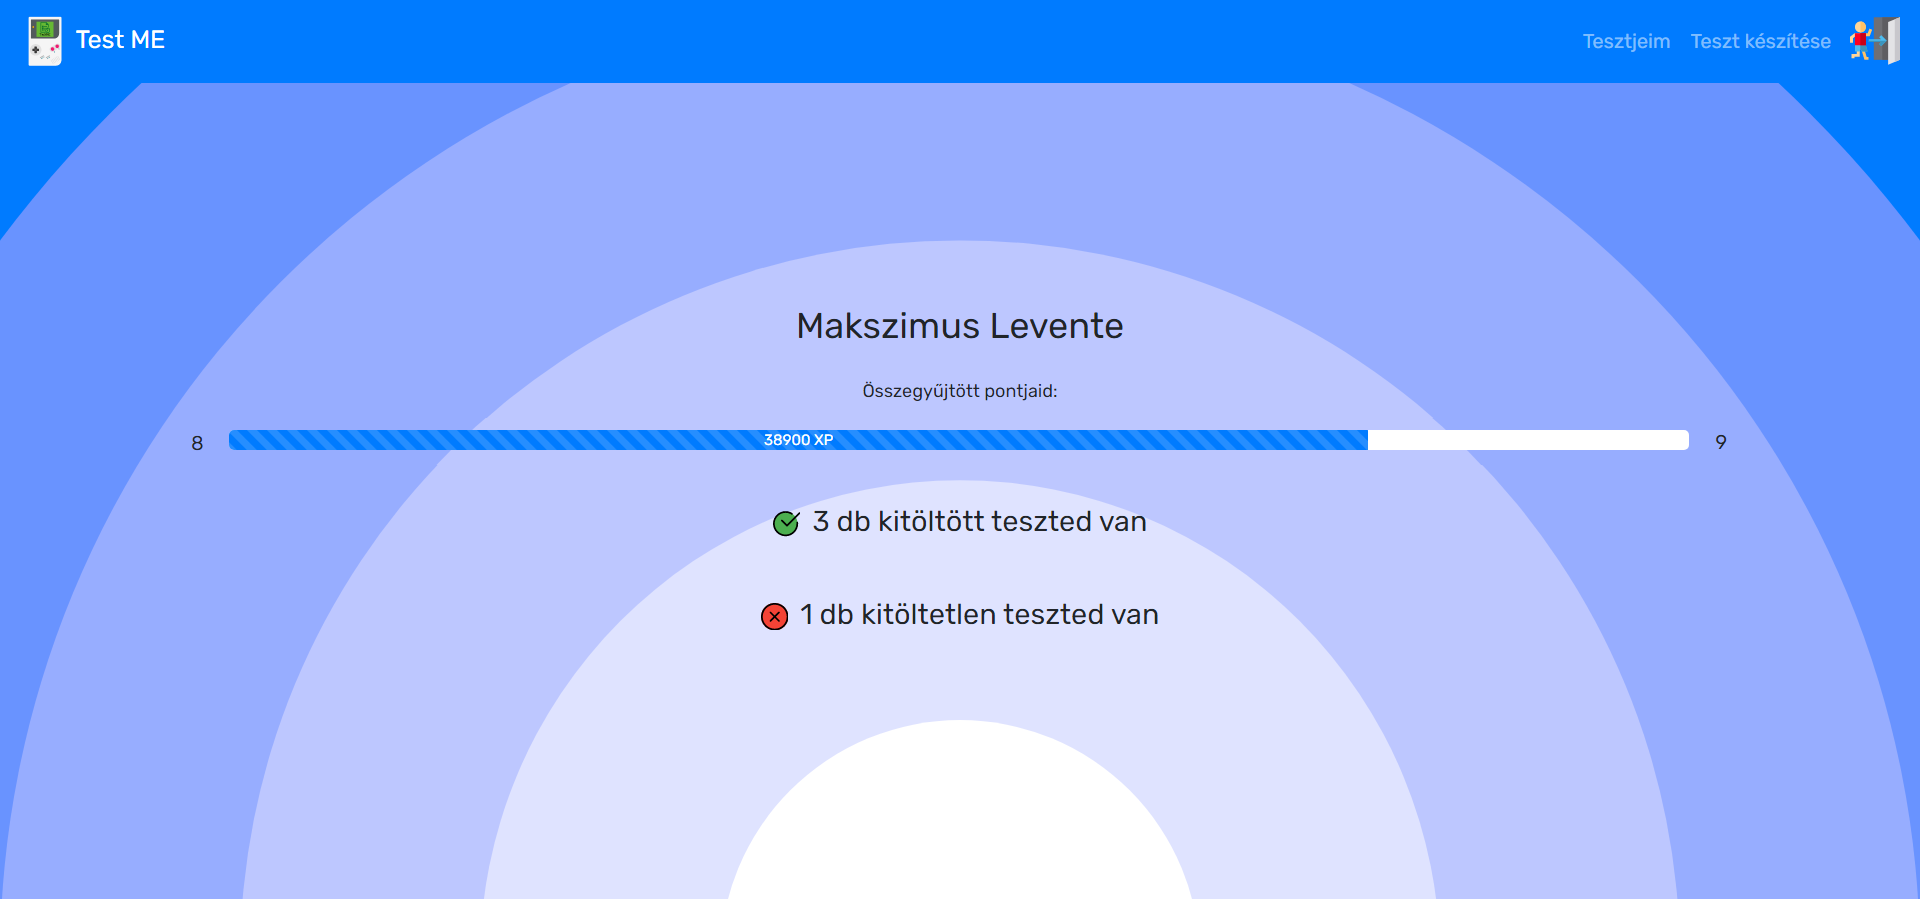
\includegraphics[width=\linewidth]{images/home.png}
    \caption{Főoldal}
\end{figure}

Bejelentkezés után automatikusan átkerülünk a főoldalra ahol láthatjuk a teljes nevünket, hanyas szintűek vagyunk a pontjaink alapján, és hogy hány darab kitöltött és kitöltetlen tesztünk van. Itt láthatjuk egyben a főbb fontos adatokat. A szint meghatározása úgy történik hogy 5000 pontoként lehet egy szintet lépni, tehát például az itt szereplő képen 8 és 9-es szint között vagyok. Ez azt jelenti hogy 35000-től több de 40000-től kevesebb pontom van.

\subsubsection{CreateTest}

Ebben a komponenseben történik a tesztek létrehozása.

\begin{figure}[H]
    \centering
    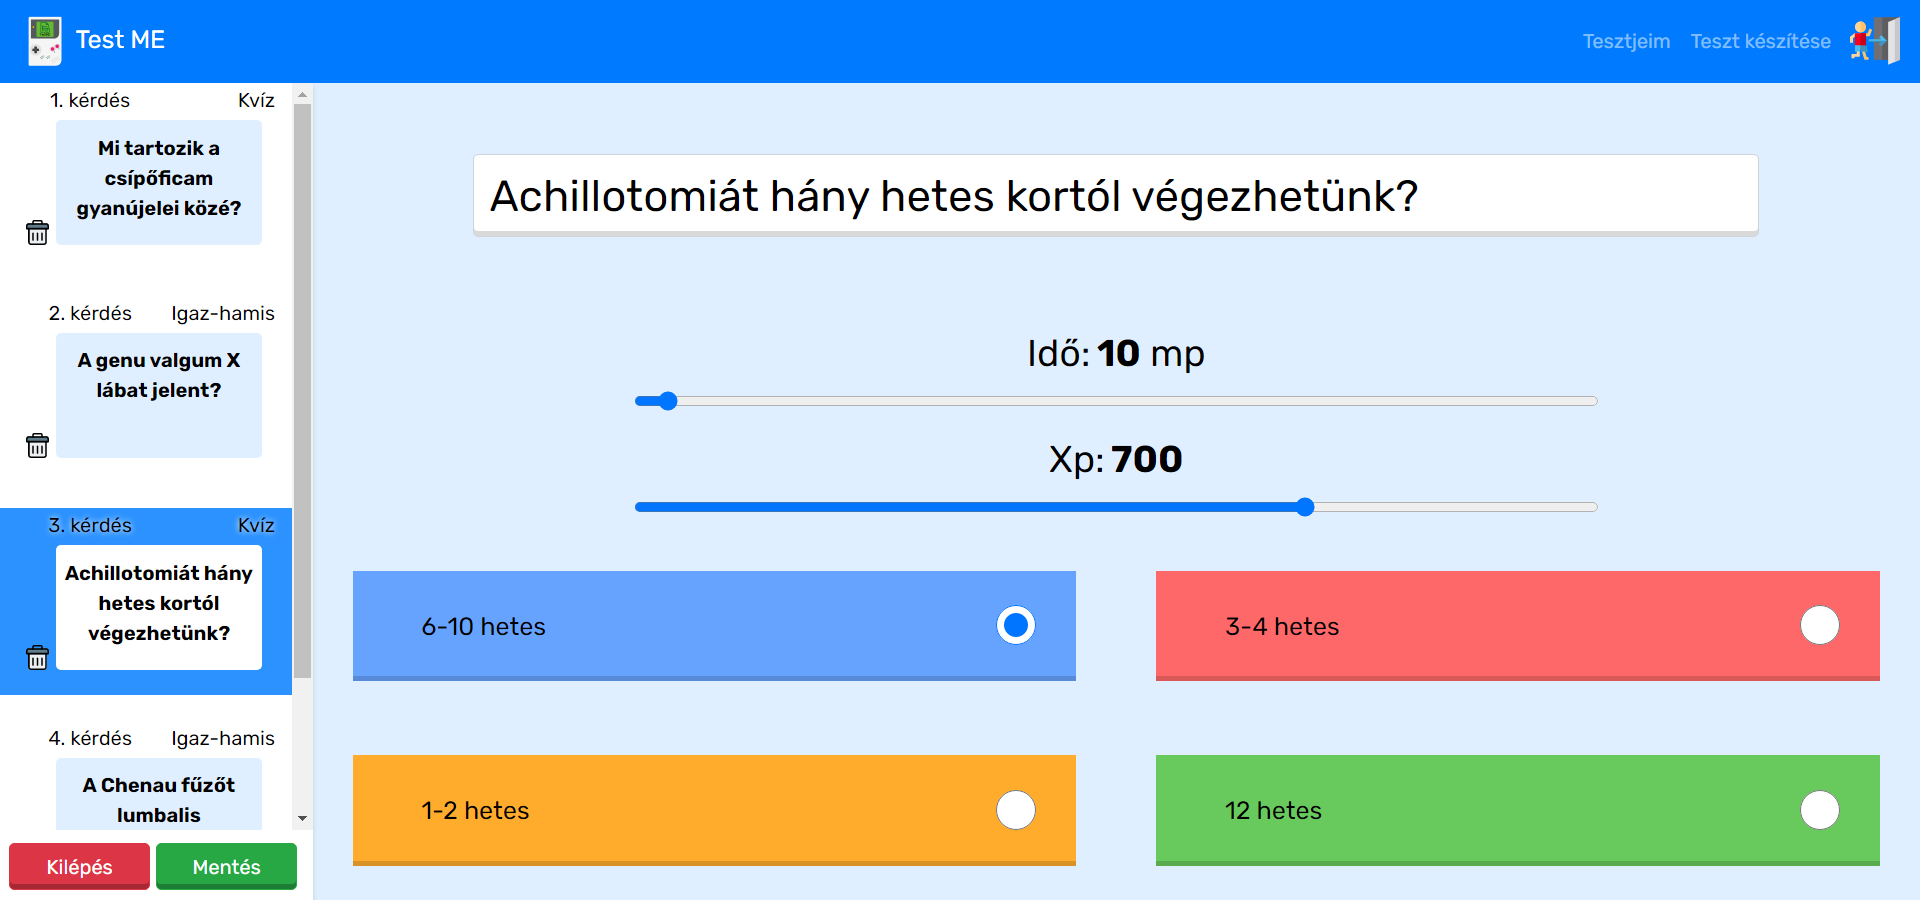
\includegraphics[width=\linewidth]{images/make_test1.png}
    \caption{Teszt készítés}
\end{figure}

Két részre van osztva a felület. A bal oldali sávban vannak az eddig hozzáadott kérdéseink amiket tudunk létrehozni, törölni, kiválasztani majd szerkeszteni. A téglalapokban látszódik a feltett kérdésünk, fölötte pedig hogy hányadik és hogy milyen típusú. A jobb oldali részen pedig ha rákattintunk egy létrehozott kérdésre ide tölti be a kérdés adatait és így tudjuk kitölteni vagy módosítani. Itt adjuk meg hogy mi legyen a kérdés, mik a lehetséges válaszok, ezek közül melyik a jó, mennyi időt engedünk hogy válaszoljanak rá és hogy mennyi pontot adunk érte. Ez a pont viszont teszt kitöltésnél idő és válasz alapján dől el hogy mennyit kap belőle a kitöltő. Tehát például ezt a 700 pontot akkor kaja meg ha azonnali jó választ ad, minél többet gondolkodik a kérdésen annál kevesebbet kap meg belőle. Tehát itt, a maximum pontot kell meghatározni.

\begin{figure}[H]
    \centering
    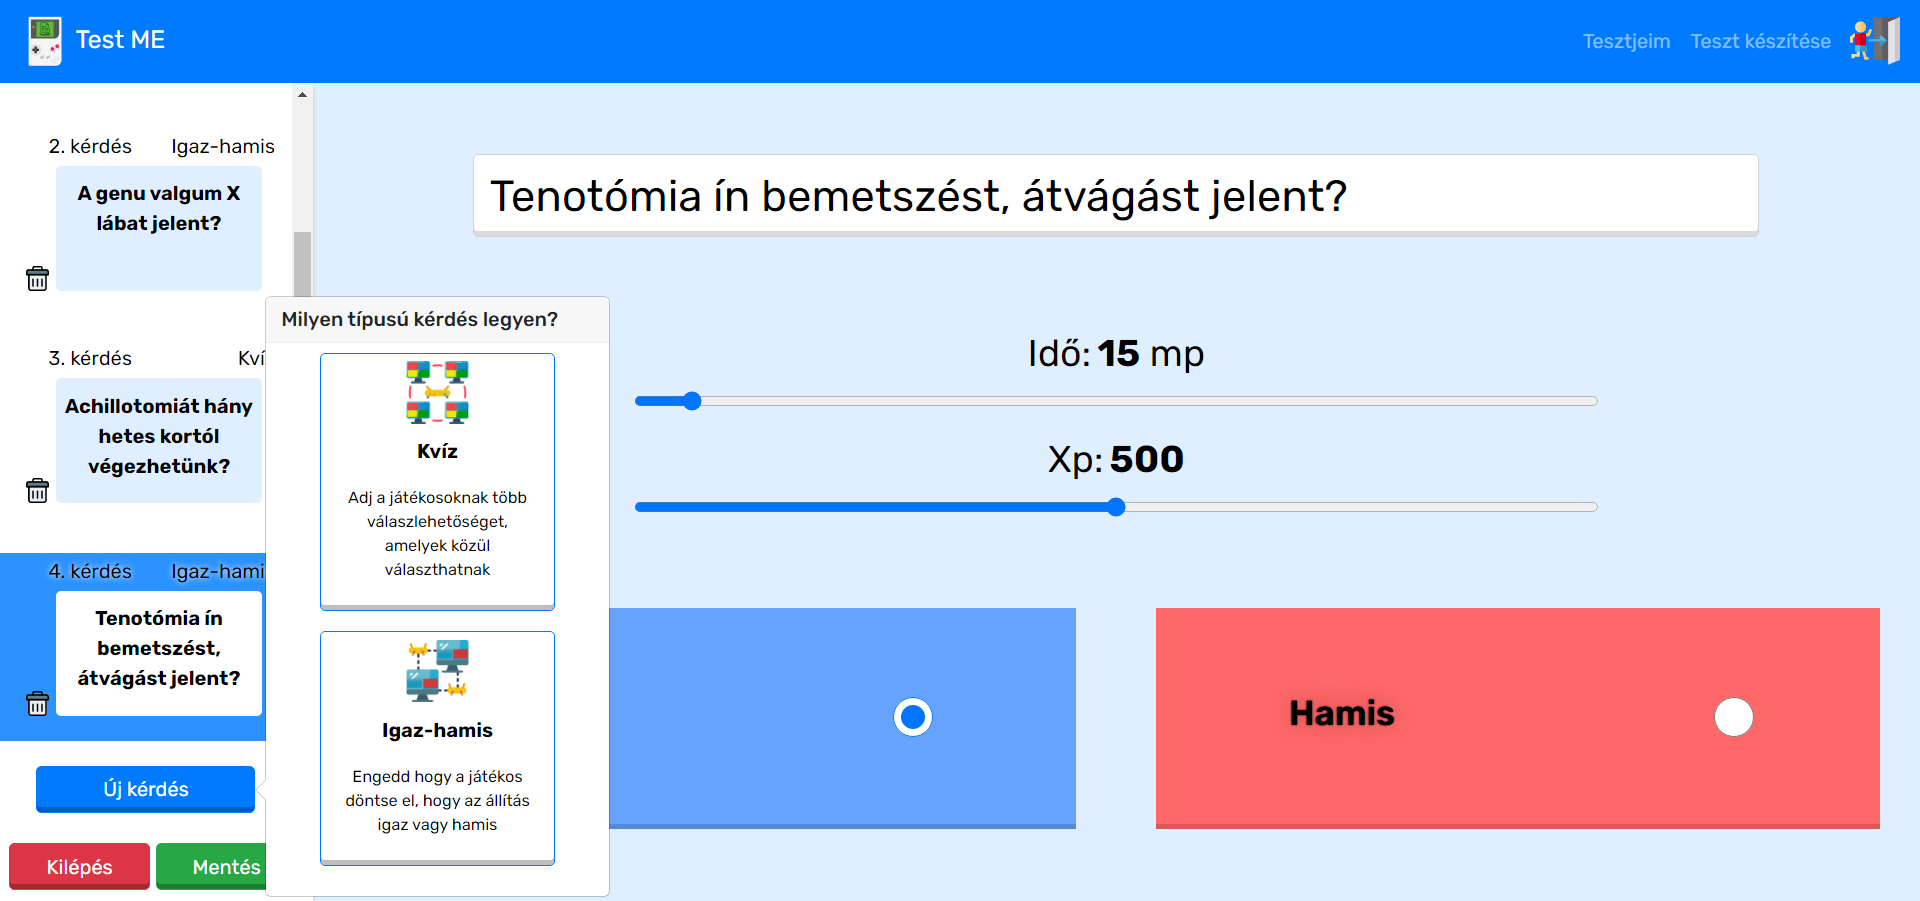
\includegraphics[width=\linewidth]{images/make_test2.png}
    \caption{Kérdés típus választás}
\end{figure}

Kétféle kérdés típus közül lehet választani. Van a kvíz kérdés, aminél egy kérdésre négy válaszlehetőség van és egy jó válasz. Valamint van az igaz-hamis aminél értelem szerűen meg kell adni hogy a feltett kérdés igaz vagy hamis.


\begin{figure}[H]
    \centering
    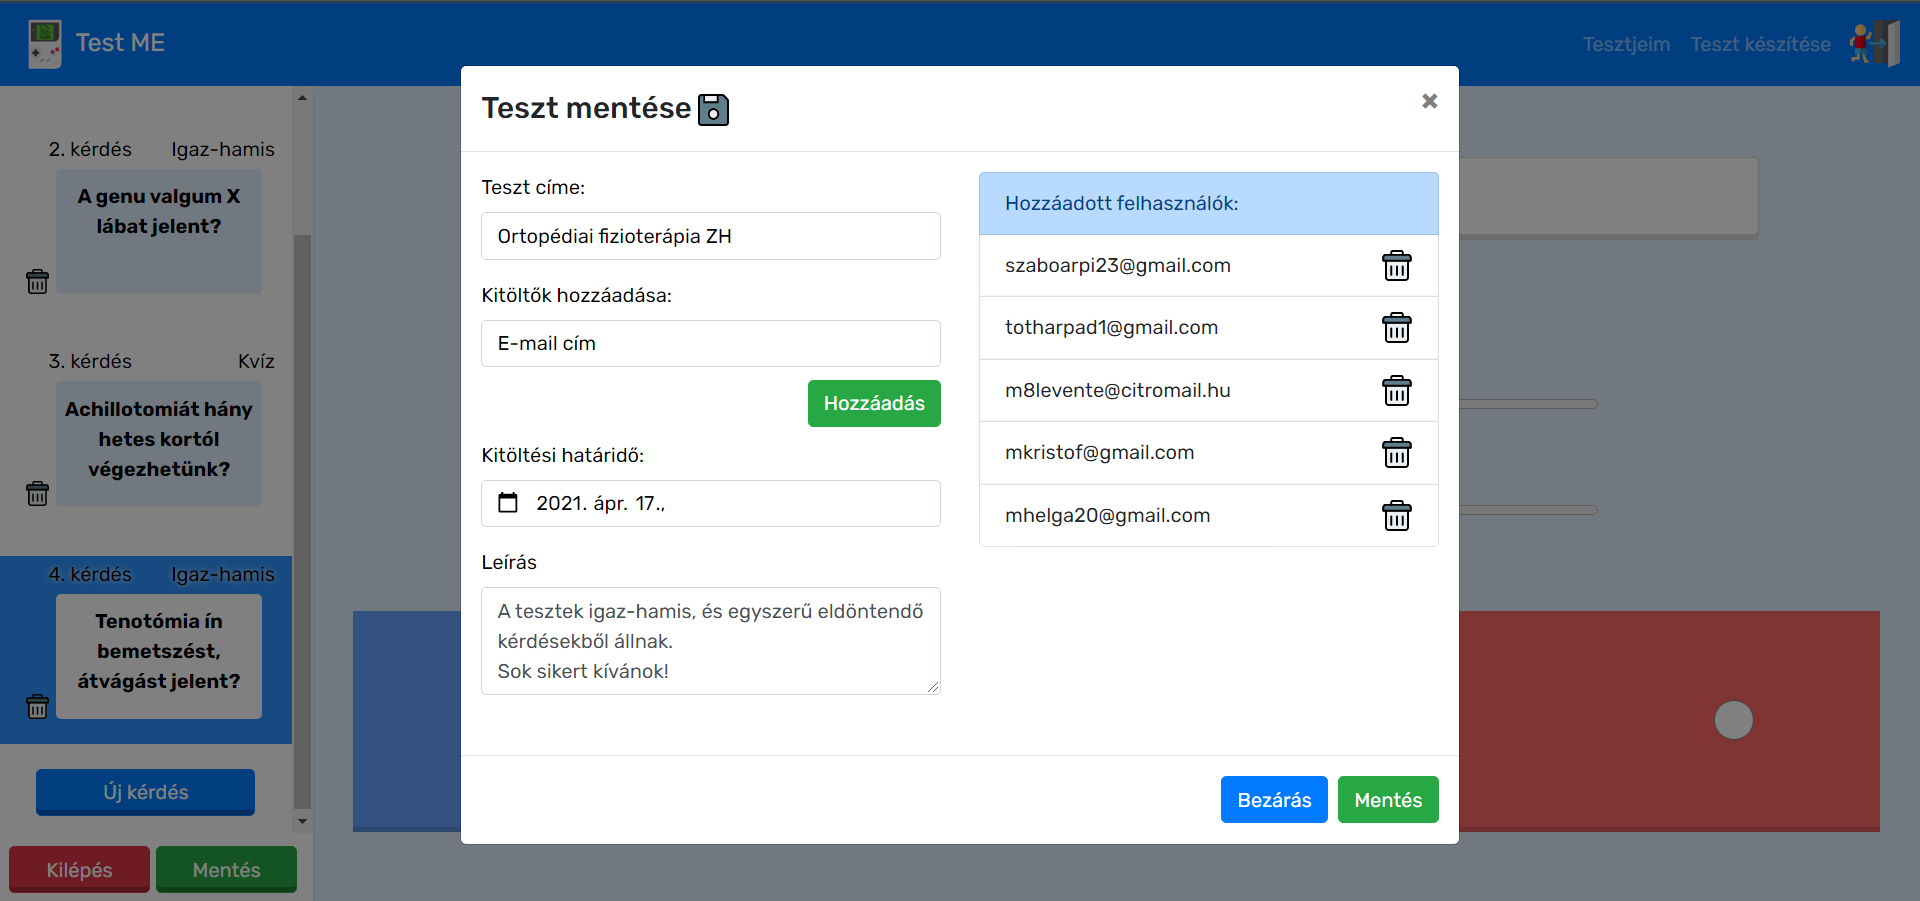
\includegraphics[width=\linewidth]{images/make_test3.png}
    \caption{Teszt mentése}
\end{figure}

Ezután ha mindennel megvagyunk és rákattintunk a mentés gombra, majd felugrik egy űrlap ahova be kell írni az alap teszthez tartozó adatokat. Ezek közé tartozik a teszt címe, kitöltési határideje, leírása és a felhasználók email címe, akiknek ki kell töltenie a tesztet. Az utóbbit úgy tudjuk megtenni hogy beírjuk a mezőbe és a hozzáadás gombbal tudjuk hozzáadni az oldalsó listához, valamint törölni is tudjuk őket ha véletlenül rosszul írtunk volna be egy email-t.

\subsubsection{MyTests}


\begin{figure}[H]
    \centering
    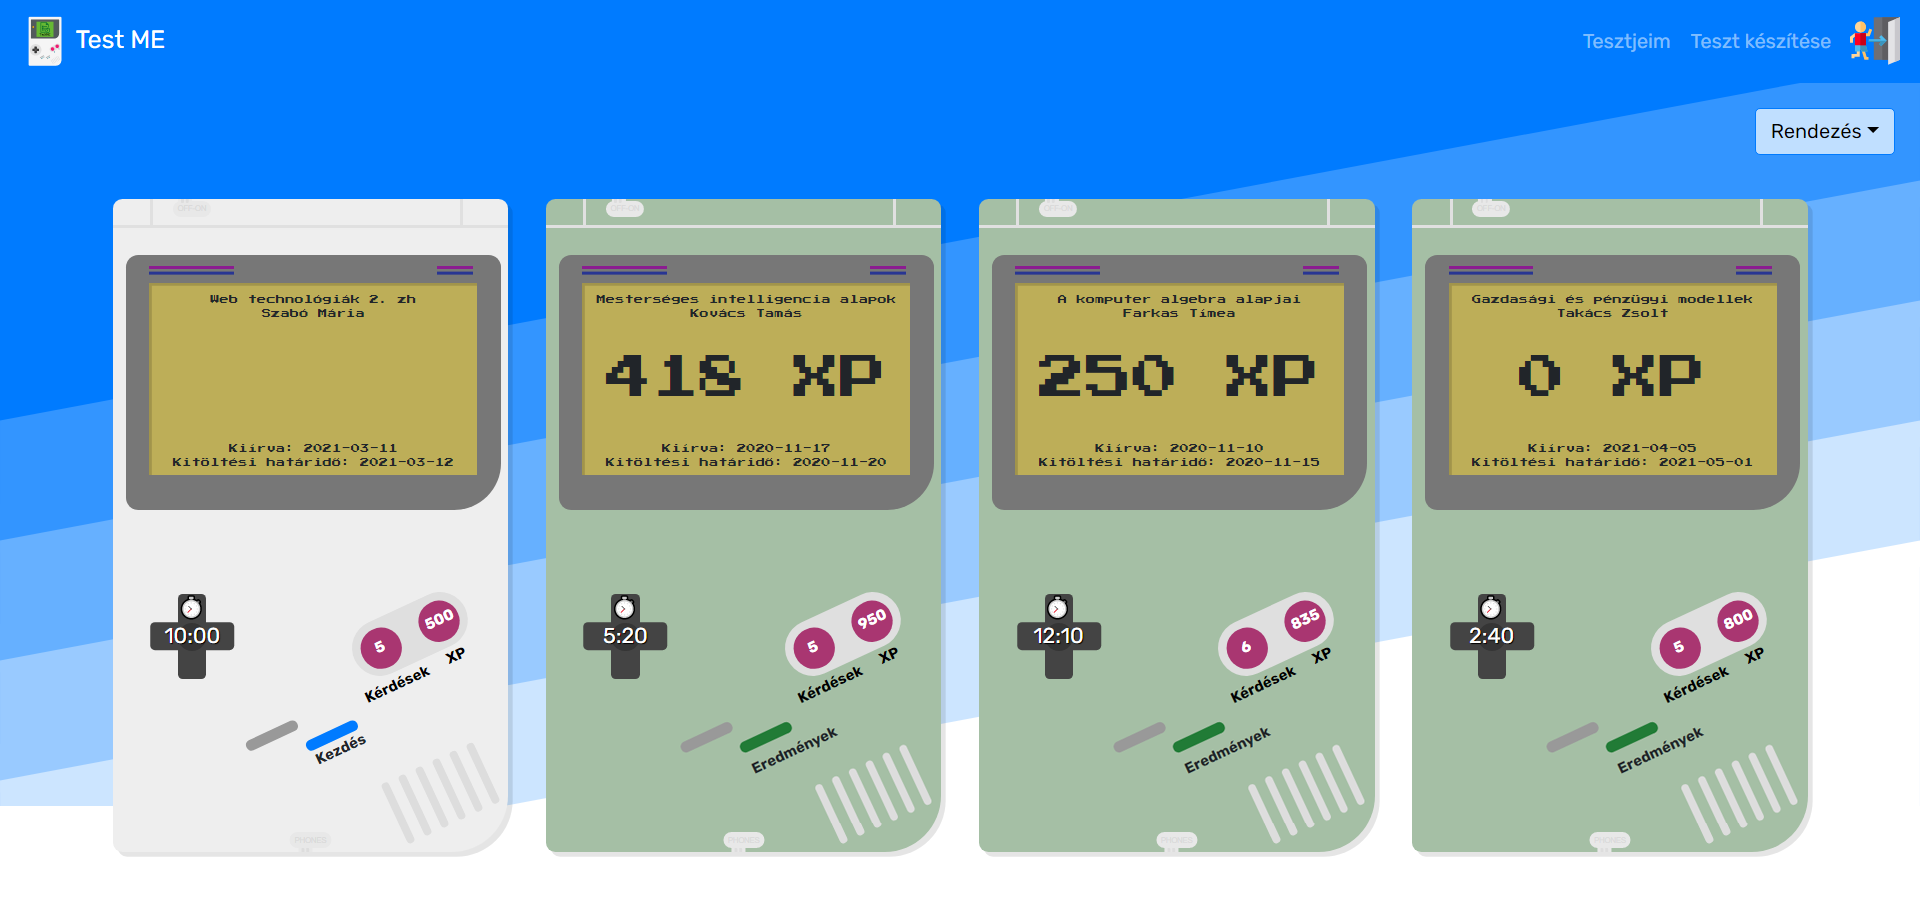
\includegraphics[width=\linewidth]{images/my_tests.png}
    \caption{Saját tesztek}
\end{figure}

Azután hogy elmentettük a tesztet átkerülünk a "Tesztjeim" nevű oldalra, ahol megnézhetjük a tesztjeinket amiket ki kell töltenünk vagy amiket mi hoztunk létre. Itt a játékosság szemléltetése végett minden tesztet egy Game Boy ábrázol. Itt látszódik rajta a teszt címe, hogy ki készítette és mikor, mi a kitöltési határidő, mennyi idő van az összes kérdésre egybevéve, hány kérdés van, és hogy mennyi pont jár az az összes kérdésre ha hibátlanul és gyorsan válaszolunk.

Azt hogy melyik kérdést hoztuk mi létre és melyik az amelyiket nekünk kell kitölteni, azt két helyen is észre lehet venni. Először is látjuk hogy a teszt címe alatt a saját nevük van, második pedig hogy a "Kezdés" gomb helyett rögtön azt látjuk hogy "Eredmények". Viszont ugyan ez az "Eredmények" gomb lesz ott akkor is, ha egy tesztet már kitöltöttünk és később vissza szeretnénk nézni hogy mások hogy teljesítettek. Igy össze tudjuk hasonlítani az eredményünket másokéval, de elsősorban ez a teszt kitöltőjének jelent fontos információt az, hogy ki hány pontot szerzett.

A kérdéseket tudjuk rendezni is úgy hogy a legújabb vagy a legrégebben kiírt teszt legyen elől vagy hogy a kitöltetlenek legyenek az elsők.
A kitöltött tesztek kitöltés után zöld színűek lesznek és a Game Boy kijelzőjén látjuk az elért pontunkat.


\subsubsection{CompleteTest}

Ha rákattintunk a teszteknél a kezdés gombra elindul a teszt kitöltése és betöltődik a CompleteTest komponens. A CompleteTest-nek 3 további gyerek elemi vannak. Az egyik a QuestionType, ez az ami megjelenik a kérdés előtt hogy segítse a felhasználót. A következő maga a kérdés ami a kérdést hozza fel a válaszlehetőségekkel, legyen az igaz-hamis vagy kvíz. Az utolsó pedig az Results ami az eredményeket sorolja fel. A CompleteTest pedig ezeket a komponenseket váltogatja addig amíg véget nem ér a teszt.

\begin{figure}[H]
    \centering
    
\includegraphics[width=\linewidth]{images/question_type.png}
    \caption{Válaszadás előtt a kérdés}
\end{figure}

Azért hogy a kitöltőnek legyen ideje felkészülni egy kérdésre, mindegyik előtt bejön a típusa amit egy képpel jelzek és alatta a kérdés szövege. Így hogy el tudja olvasni válaszadás előtt, van lehetősége a felhasználónak gyorsan is válaszolni és jó pontot kapni a rá. A kérdés alatt pedig megy egy visszaszámláló hogy mennyi ideje van még elolvasni.

\begin{figure}[H]
    \centering
    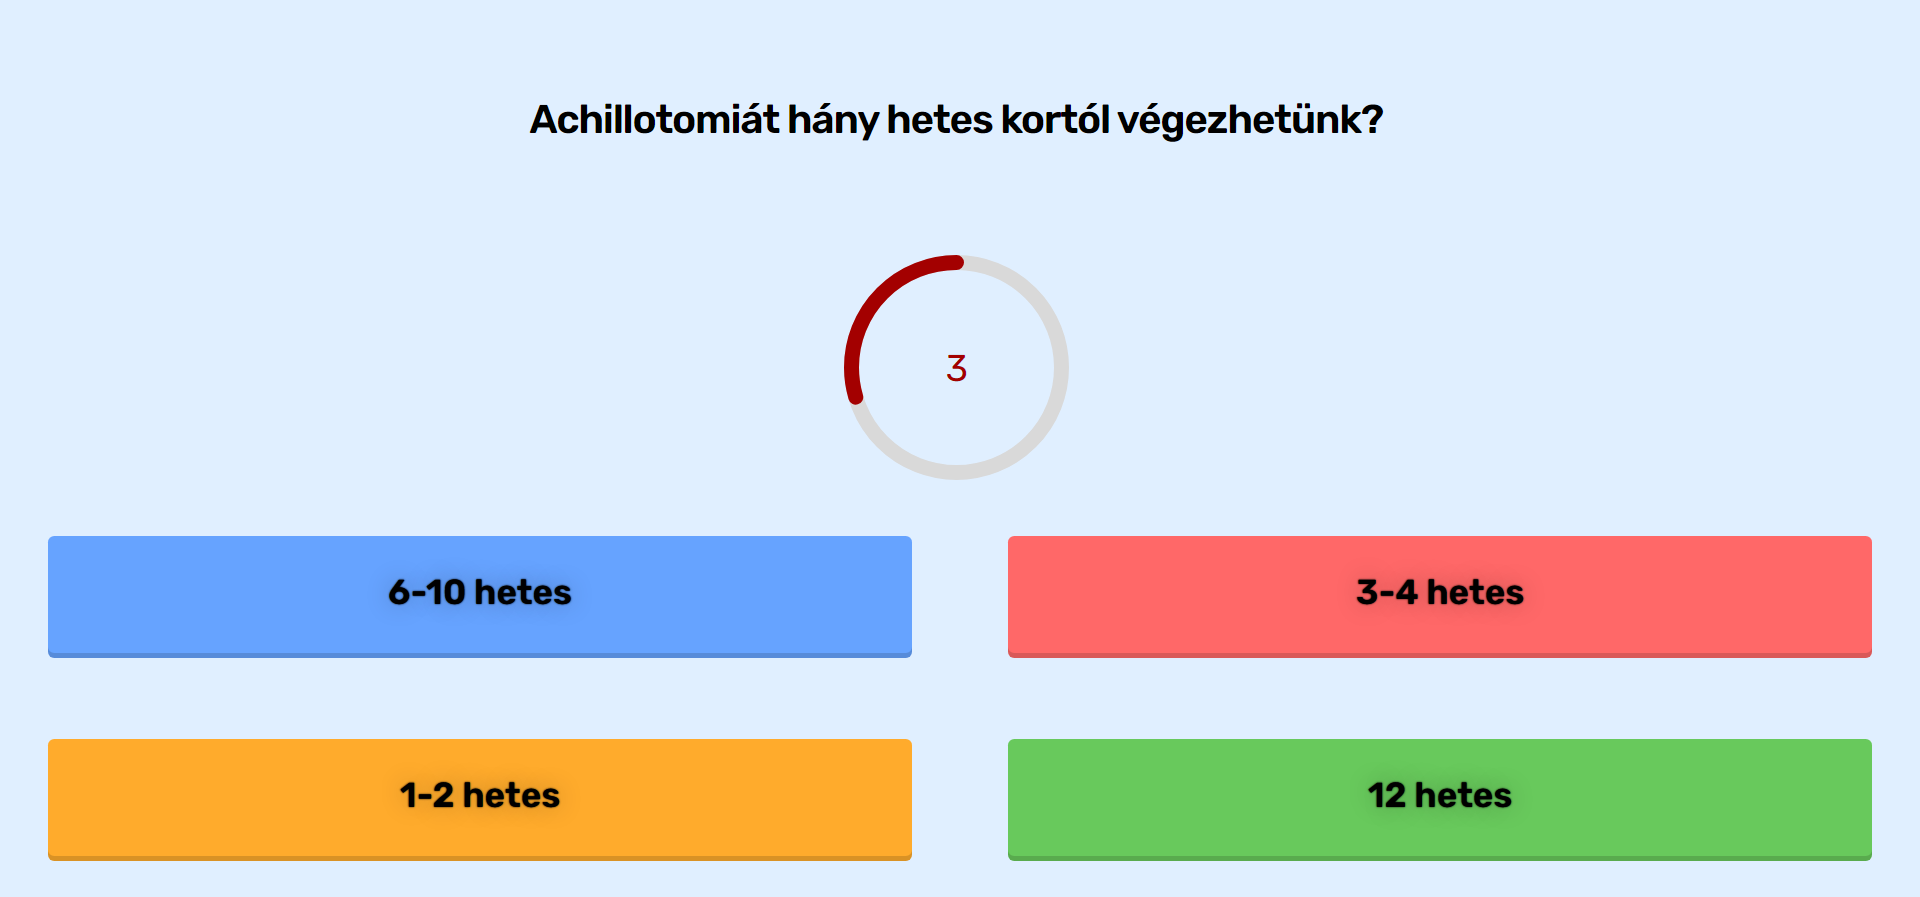
\includegraphics[width=\linewidth]{images/question1.png}
    \caption{Kvíz kérdés}
\end{figure}

Majd ezután bejön a kérdés újra viszont a négy válasszal együtt. Itt is megy a visszaszámláló, minden kérdésnél annyi másodperctől kezdődik a visszaszámlálás amennyit a tesztkészítő megadott a konkrét kérdésre.

\begin{figure}[H]
    \centering
    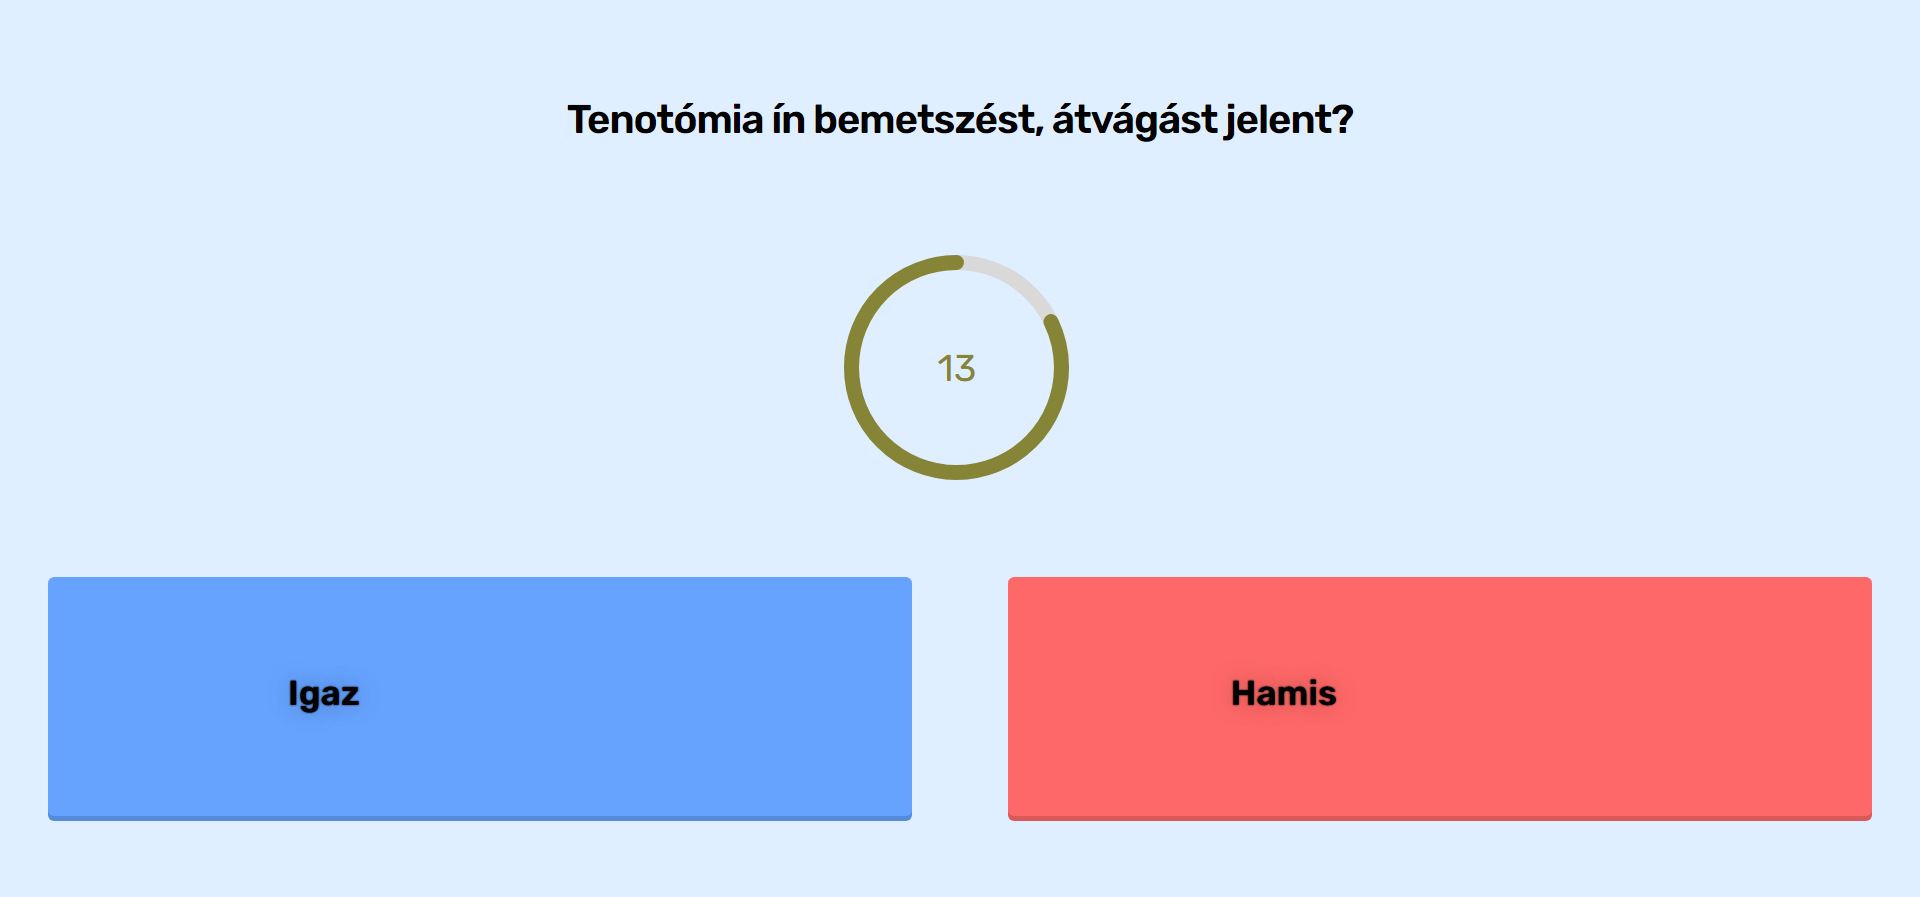
\includegraphics[width=\linewidth]{images/question2.png}
    \caption{Igaz-hamis kérdés}
\end{figure}

Egy igaz-hamis kérdés is ugyan így működik, viszont csak 2 lehetőség van.


\begin{figure}[H]
    \centering
    \begin{subfigure}{0.5\textwidth}
        \centering
        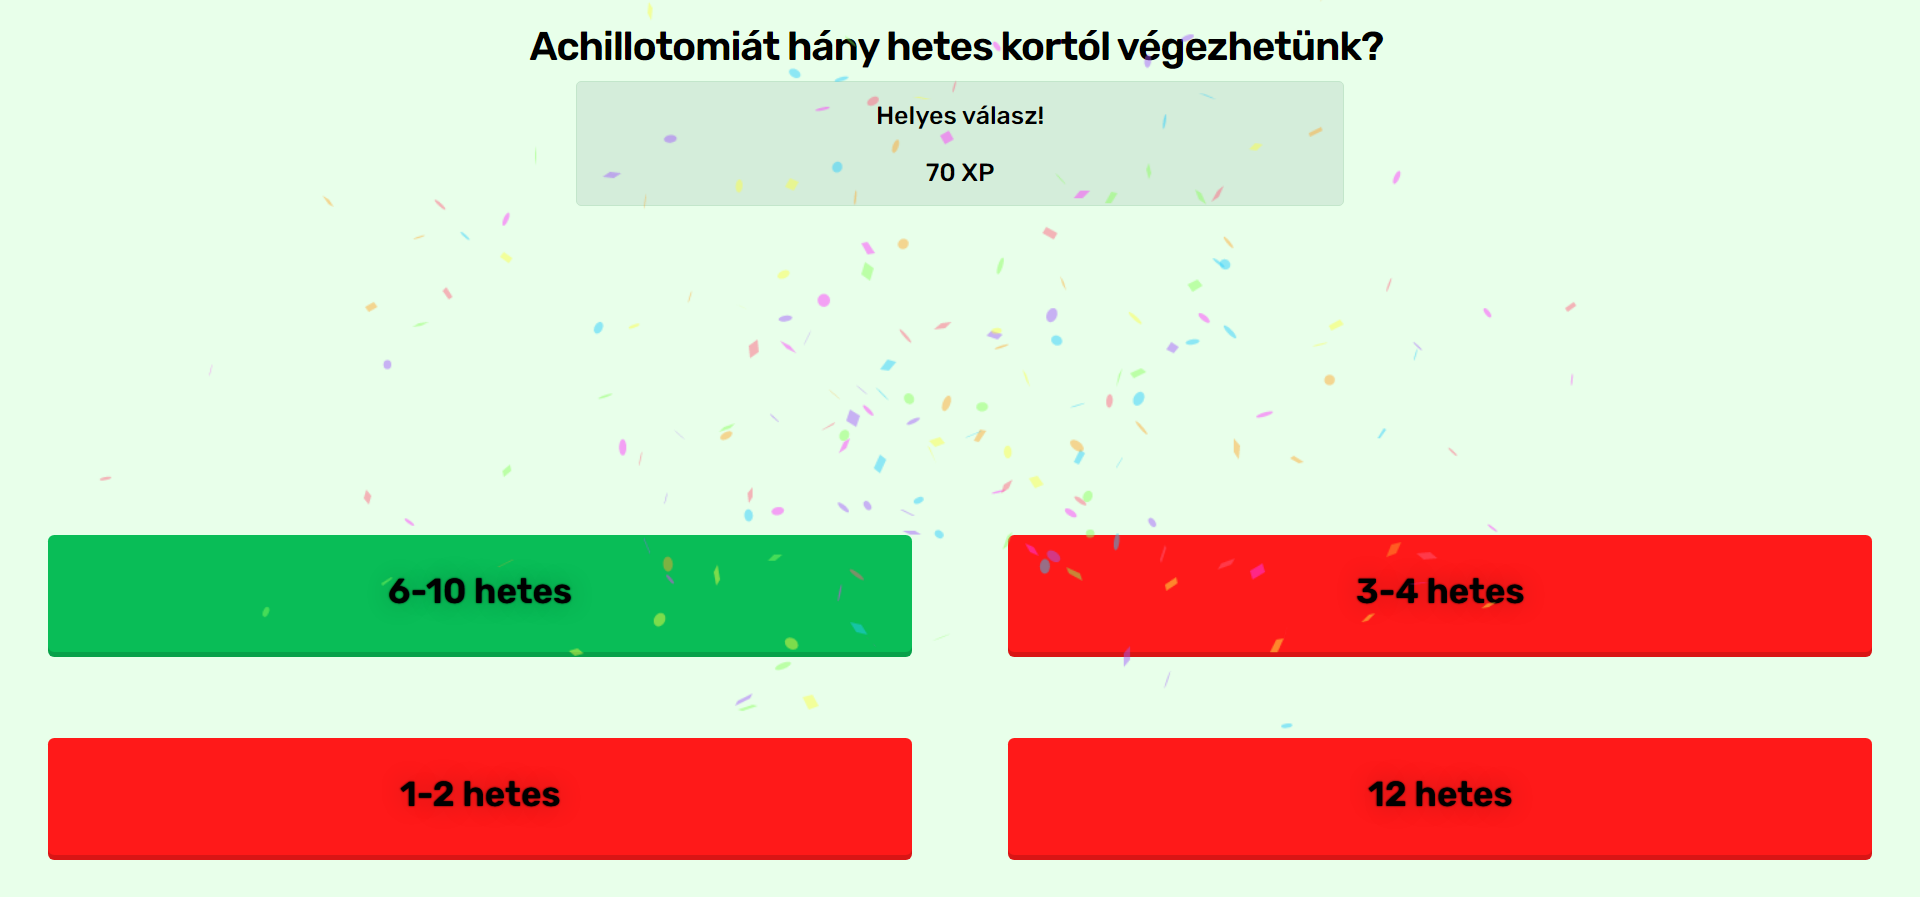
\includegraphics[width=\linewidth]{images/question_good.png}
        \caption{Jó válasz}
        \label{fig:sub1}
    \end{subfigure}%
    \begin{subfigure}{0.5\textwidth}
        \centering
        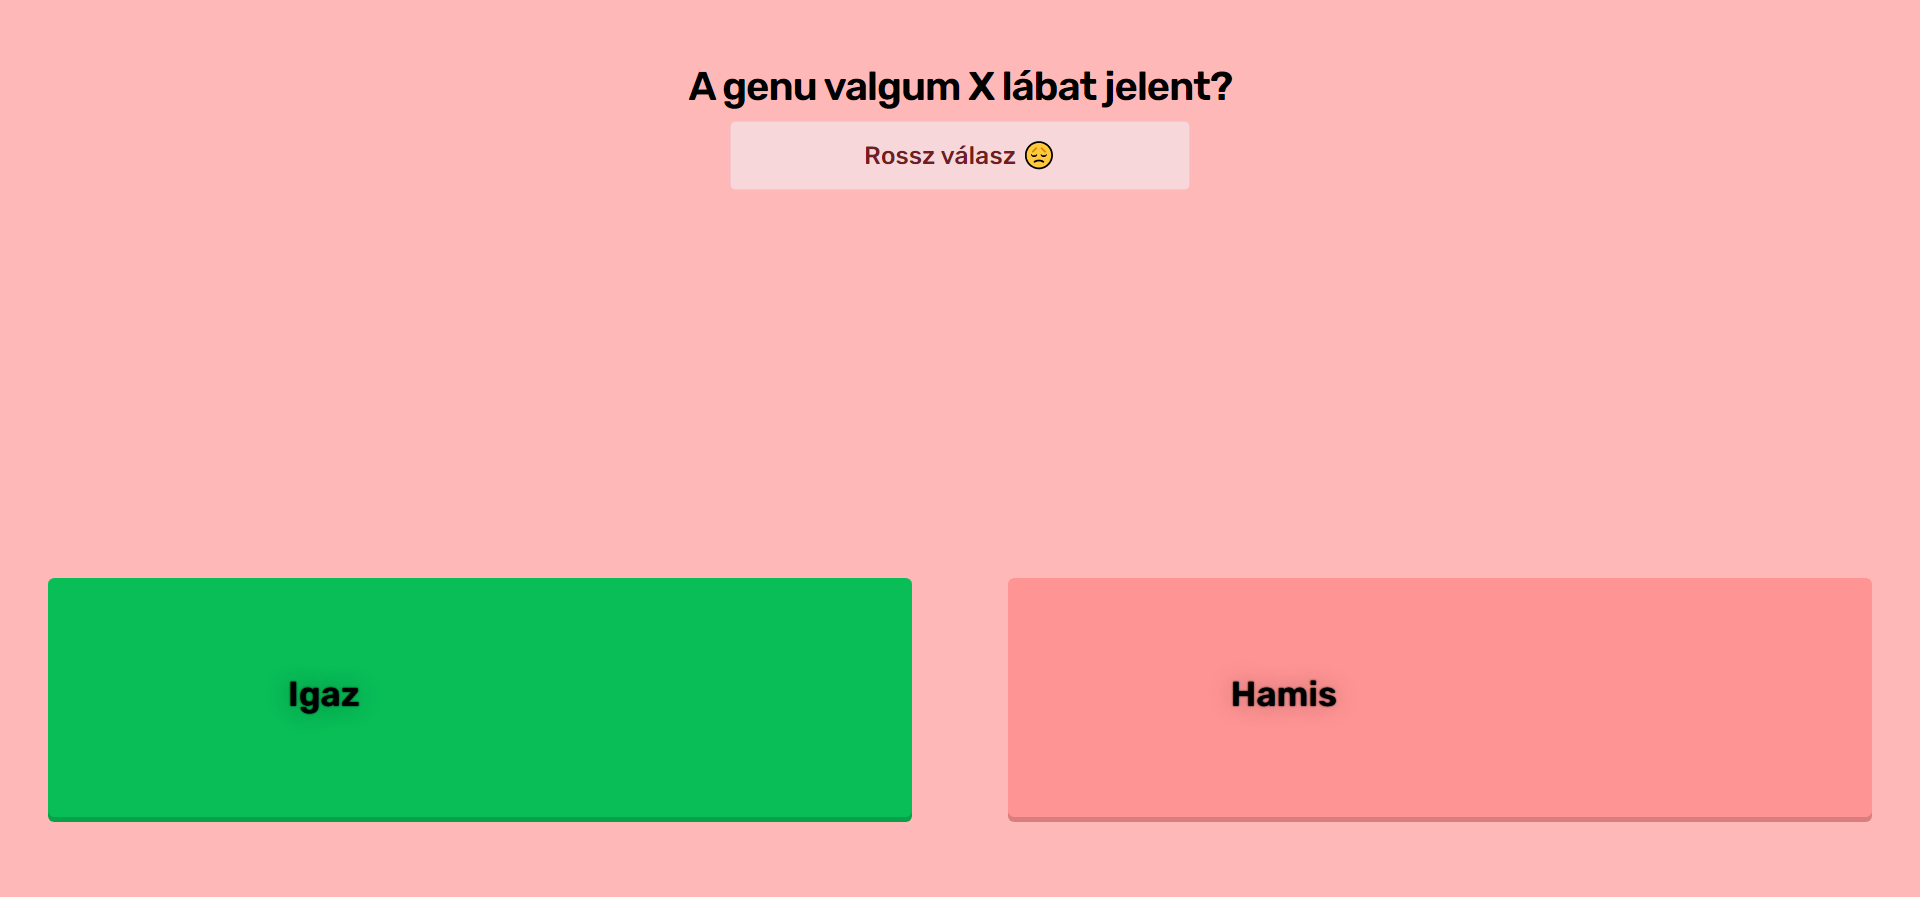
\includegraphics[width=\linewidth]{images/question_wrong.png}
        \caption{Rossz válasz}
        \label{fig:sub2}
    \end{subfigure}
    \caption{Válaszadás}
    \label{fig:test}
\end{figure}

Egy kérdés 3 féleképpen fejeződhet be. Az első az, ahogy a kép is mutatja, hogy jó választ kapunk a kérdésre és megkapjuk a kiérdemelt pontot. A második hogy rosszul válaszolunk és nem kapunk semmit. Az utolsó pedig hogy nem válaszolunk, ilyenkor az idő lejárta után, autómatikusan rossz válasznak veszi a rendszer és tovább lép a következő kérdésre.

Az XP értéke a helyesség és a sebesség alapján számolódik ki.
Jó válasz esetén a pontszámítás az alábbi képlet szerint működik:
\[ \left\lfloor\left(\frac{\left(\frac{\left( időkorlát - maradék idő\right)}{ időkorlát}\right)}{2}\right)\cdot xp\right\rfloor \]
Viszont ha azonnali jó választ adunk, akkor a képleten látható számítás nem megy végbe, hanem megkapjuk az összes lehetséges pontot amit a kérdésre lehet.


\begin{figure}[H]
    \centering
    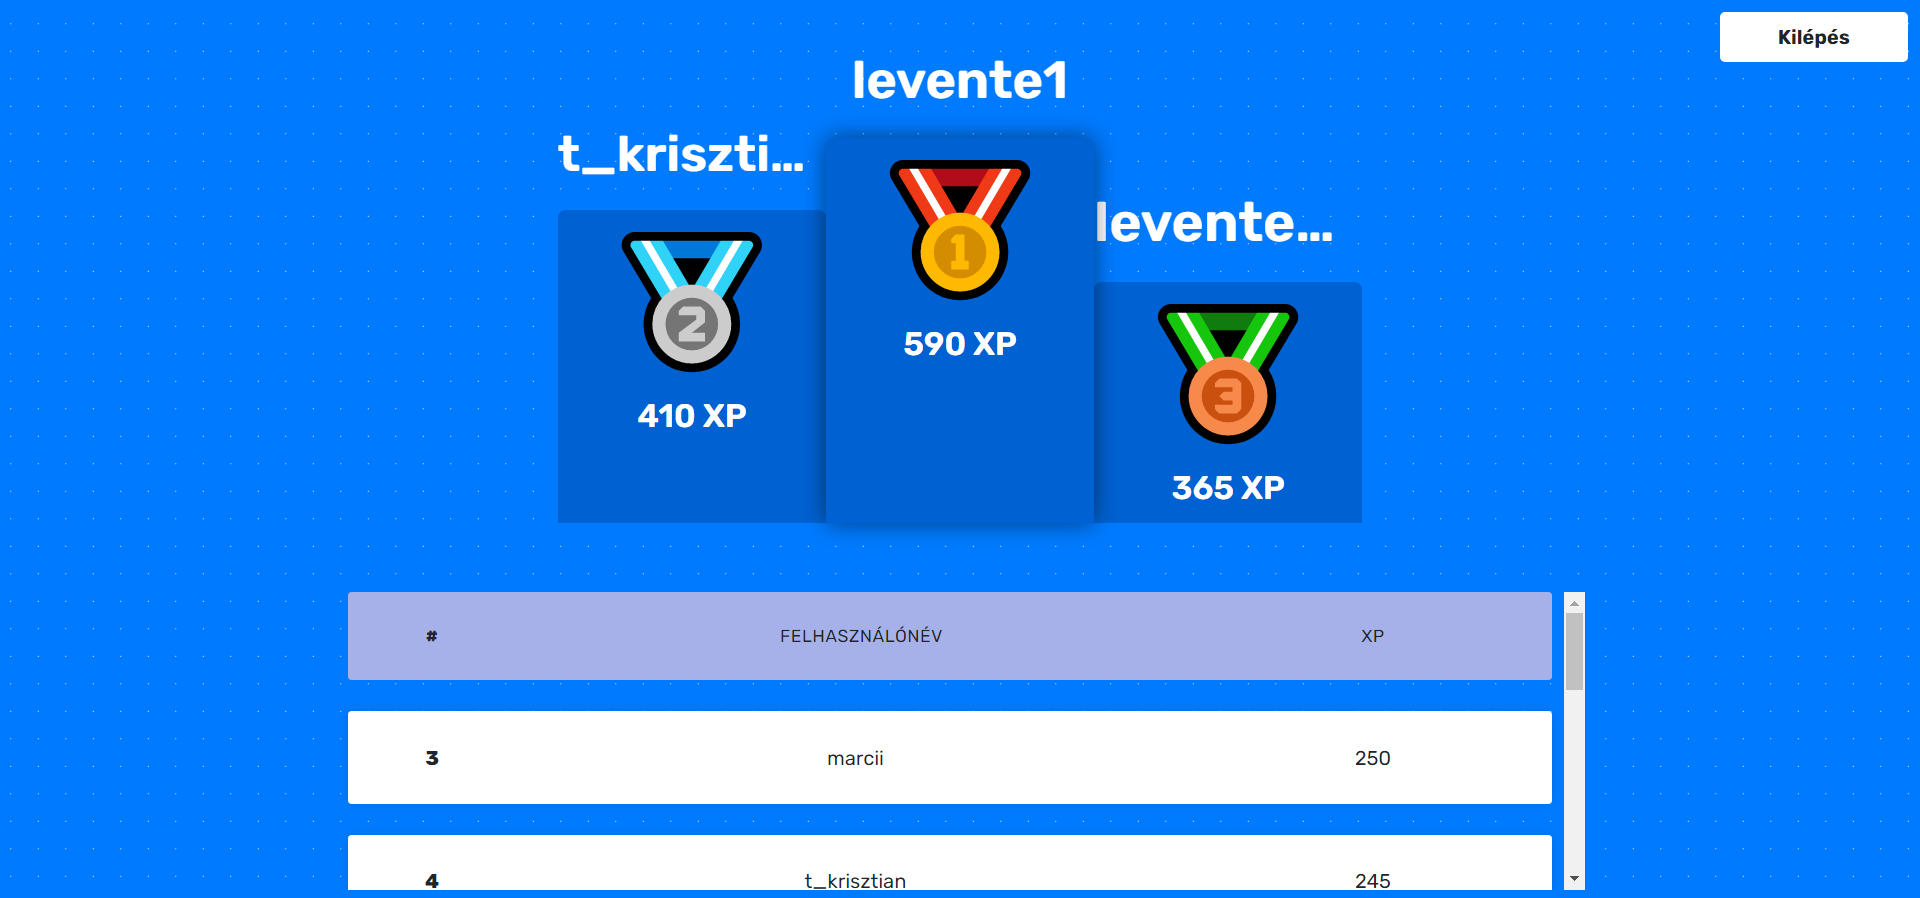
\includegraphics[width=\linewidth]{images/results.png}
    \caption{Eredmények a teszt után}
\end{figure}

Majd ha az összes kérdés elfogyott, összeadjuk a felhasználó összesen elért pontját és megjelenítjük a többiekével együtt. Így megnézhetjük hogy hányadikok lettünk. Ezután a "Kilépés" gombra kattintva vissza kerülünk a tesztjeinkhez és a főoldalon látjuk hogy több pontunk lett, ha értünk el pontot a teszt kitöltése során.